\documentclass[10pt,a4paper]{article}
\usepackage[utf8]{inputenc}
\usepackage[T1]{fontenc}
\usepackage[ngerman]{babel}
\usepackage{amsmath}
\usepackage{amsfonts}
\usepackage{amssymb}
\usepackage{graphicx}


\author{Gruppe 02}
\title{Pflichtenheft}
\begin{document}
% Title Page foo
\maketitle
% Inhaltsverzeichniss
\tableofcontents
%------------------------------------------------
% Zielbestimmung
%------------------------------------------------
\section{Zielbestimmung}
	\subsection{Musskriterien}
	\begin{itemize}
		\item Webanwendung
		\begin{itemize}
			\item Es gibt eine \emph{Startseite}, welche am Corporate Design der Universität und der klik-Webseite orientiert ist.
                        \item Über die Startseite können sich Benutzer einloggen oder neu registrieren.
			\item Ohne Anmeldung sind ausschließlich die Startseite und die Liste aller Aktivitäten einsehbar.
			\item Bei der Registrierung \emph{müssen} Vorname, Nachname, eine Universitäts-Email-Adresse und Studiengang bzw. Dienststelle angegeben werden.
                        \item Nach jeder Anmeldung werden Benutzer auf ihre \emph{Landingpage} weitergeleitet.
                        \item Benutzer können ihrem Profil ein individuelles Bild hinzufügen, welches auf der Landingpage und der Profilseite als Avatar angezeigt wird.
                        \item Benutzer sammeln Punkte, und können diese auf ihrer \emph{Landingpage} einsehen. 
                        \item Benutzer können über ihre Landingpage neue Teams erstellen um gemeinsam mit anderen Benutzern Punkte zu sammeln.
                        \item Der Punktestand eines Teams berechnet sich als Mittelwert der Punktestände aller Benutzer des Teams.
                        \item Jeder Teilnehmer und jedes Team hat eine \emph{Profilseite}, welches von anderen Benutzern eingesehen werden kann.
                        \item Eine Profilseite zeigt den aktuellen Punktestand, die aktuell ausgewählten Aktivitäten, die abgeschlossenen Aktivitäten und ggf. ein individualisiertes Profilbild (s. Sollkriterien) des Benutzers oder des Teams.
                        \item Über die Profilseite eines Teams können Benutzer dem Team beitreten.
                        \item Jeder Benutzer kann höchstens in \emph{einem} Team Mitglied sein.
                        \item Benutzer können andere Benutzer in \emph{ihr} Team einladen. Einladungen in fremde Teams sind nicht möglich.
			\item Benutzer können Energiesparvorschläge über eine \emph{Vorschlagsseite} einreichen.
                        \item Ein Energiesparvorschlag besteht aus einer Bezeichnung.
                        \item Auf der Vorschlagsseite wird außerdem eine Übersicht über alle von allen Benutzern bisher eingereichten Energiesparvorschläge dargestellt.
                        \item Über die Vorschlagsseite können Benutzer Energiesparvorschläge kommentieren und/oder mit 1 bis 5 Sternen bewerten.
			\item Benutzer können Aktivitäten (s. Adminbereich) über eine \emph{Aktivitätsseite} auswählen und als erledigt markieren.
                        \item Um eine Aktivität als erledigt zu markieren ist eine zusätzliche Bestätigung erforderlich.
			\item Alle Benutzer nehmen an allen Challenges automatisch teil.
			\item Es gibt eine nach Punktestand sortiert Übersicht über alle Benutzer oder alle Teams (\emph{Rangliste}). In der Übersicht kann auf einfache Weise zwischen der Anzeige von einzelnen Benutzern oder Teams umgeschaltete werden.
                        \item Benutzer können über diese Rangliste nach anderen Benutzern oder Gruppen suchen.
			\item Es gibt eine \emph{Statistikseite}, die von allen Benutzern eingesehen werden kann, mit folgenden grafischen, anonymisierten Statistiken:
			\begin{itemize}
				\item Besucherzahl
				\item gesammelte Punkte
				\item erledigte Aktivitäten
				\item beliebteste Aktivitäten
			\end{itemize}
		\end{itemize}
		% ----------------------------------------------------------------
		\item Android-App
		\begin{itemize}
			\item Benutzer müssen sich beim ersten Start mit ihrem Account anmelden. Hierfür ist eine bestehende Registrierung (über die Website) erforderlich.
			\item Benutzer können Profilseiten anderer Benutzer und Teams einsehen.
			\item Benutzer können ein Ranking von Teilnehmern oder Teams einsehen.
			\item Benutzer können eine Übersicht über alle von ihnen ausgewählte Aktivitäten einsehen. In dieser Übersicht wird außerdem eine Liste aller Aktivitäten angezeigt, über die Benutzer weitere Aktivitäten auswählen können. Außerdem können Benutzer über diese Ansicht ausgewählte Aktivitäten als erledigt markieren.
			\item Benutzer können nach anderen Benutzern oder Teams suchen. 
		\end{itemize}
		% ----------------------------------------------------------------
		\item Adminbereich
		\begin{itemize}
			\item Challenges können erstellt werden.
                        \item Challenges haben einen Start- und einen Endzeitpunkt.
			\item Aktivitäten können erstellt und bearbeitet werden.
                        \item Jede Aktivität hat eine Bezeichnung, einen zeitlichen Rahmen (angegeben als Zeitintervall), eine Häufigkeit, eine Kategorie und Punkte, welche Benutzern bei Erledigung der Aktivität auf ihrem Punktekonto gut geschrieben werden.
			\item Energiesparvorschläge können angenommen und in Aktivitäten umwandelt werden.
                        \item Durch Annahme eines Energiesparvorschlags wird der Vorschlag aus der Vorschlagstliste entfernt und ein Dialog zum Erstellen einer neuen Aktivität geöffnet. Die Felder dieses Dialogs werden dabei mit den Informationen aus dem Vorschlag vorbereitet.
			\item E-Mails an \emph{alle} Teilnehmer senden.
			\item Teilnehmer können gesperrt werden.
                        \item Gesperrte Benutzer können sich weder über die Startseite noch über die App einloggen. Bei dem Versuch sich einzuloggen wird gesperrten Benutzern ein Hinweis darauf angezeigt, dass ihr Profil gesperrt wurde.
                        \item Teams können gelöscht werden.
		\end{itemize}
	\end{itemize}
	\subsection{Sollkriterien}
	\begin{itemize}
			\item Benutzern wird nach der Registrierung eine Liste von empfohlenen Teams angezeigt. Über diese Liste können die Benutzer direkt die Profilseiten der Teams erreichen (wo sie einem Team beitreten können).
			\item Administratoren können Benutzer und Teams löschen und gesperrte Benutzer und Teams reaktivieren.
			\item Einstellbare Benachrichtigungen für App, Browser und E-Mails.
		\end{itemize}
	\subsection{Kannkriterien}
	\begin{itemize}
                        \item Administratoren können Teams und Teilnehmer \emph{verwarnen}. Diese Verwarnung wird für alle Administratoren einsehbar gespeichert. Verwarnte Benutzer erhalten eine Benachrichtung per E-Mail über die Verwarnung, aber keine Anzeige der Verwarnung auf der Website oder in der App.
			\item Administratoren können E-Mails an einzelne Benutzer oder beliebige Gruppen von Benutzern senden.
                        \item Benutzer können über die App an Challenges teilnehmen.
                        \item Benutzer können aus ihrem Team austreten und einem anderen Team (oder auch demselben wieder) beitreten.
	\end{itemize}
	\subsection{Differentierungskriterien}
	\begin{itemize}
		\item Benutzer können weder über die Website noch über die App direkt mit anderen Benutzern kommunizieren.
		\item Weder im Browser noch in der App werden Popups im wörtlichen Sinn (also sich neu öffnende Fenster) verwendet. Stattdessen werden in der App \emph{Android Notifications} zur Darstellung von Erinnerungen an ausgewählte, aber nicht erledigte Aktivitäten verwendet. Auf der Website werden Erinnerungen an ausgewählte, aber nicht erledigte Aktivitäten in einem speziellen Info-Bereich auf der Landingpage angezeigt. 
	\end{itemize}

%------------------------------------------------
% Produkteinsatz
%------------------------------------------------
\section{Produkteinsatz}
\subsection{Answendungsbereich}
\subsection{Zielgruppe}
\subsection{Betriebsbedingungen}

%------------------------------------------------
% Produktumgebung
%------------------------------------------------
\section{Produktumgebung}
\subsection{Software}
Client: 
\begin{itemize}
\item beliebiges Betriebssystem für PC-Anwendung, das Java unterstützt 
\item Internetbrowser auf aktuellem Stand 
\item Android 5 oder höher als Betriebssoftware für mobile Geräte
\end{itemize} 
Server: 
\begin{itemize}
\item Java Runtime Environment (mindestens Version 1.7) 
\item beliebiges Betriebssystem, das Java unterstützt 
\end{itemize}

\subsection{Hardware}
Client: 
\begin{itemize}
\item Rechner/Tablet/Smartphone mit Internetverbindung 
\end{itemize} 
Server: 
\begin{itemize}
\item Rechner mit Internetverbindung 
\end{itemize}

\subsection{Orgware}
\begin{itemize}
\item Administrator muss sowohl den Client als auch den Server konfigurieren
\end{itemize}


%------------------------------------------------
% Produktuebersicht
%------------------------------------------------
\section{Produkt\"ubersicht}

%------------------------------------------------
% Akteure
%------------------------------------------------
\section{Akteure}

%------------------------------------------------
% Produktfunktion
%------------------------------------------------
\section{Produktfunktion}
\subsection{Webseite}

	\subsubsection{Startseite}
	\begin{figure}[h]
		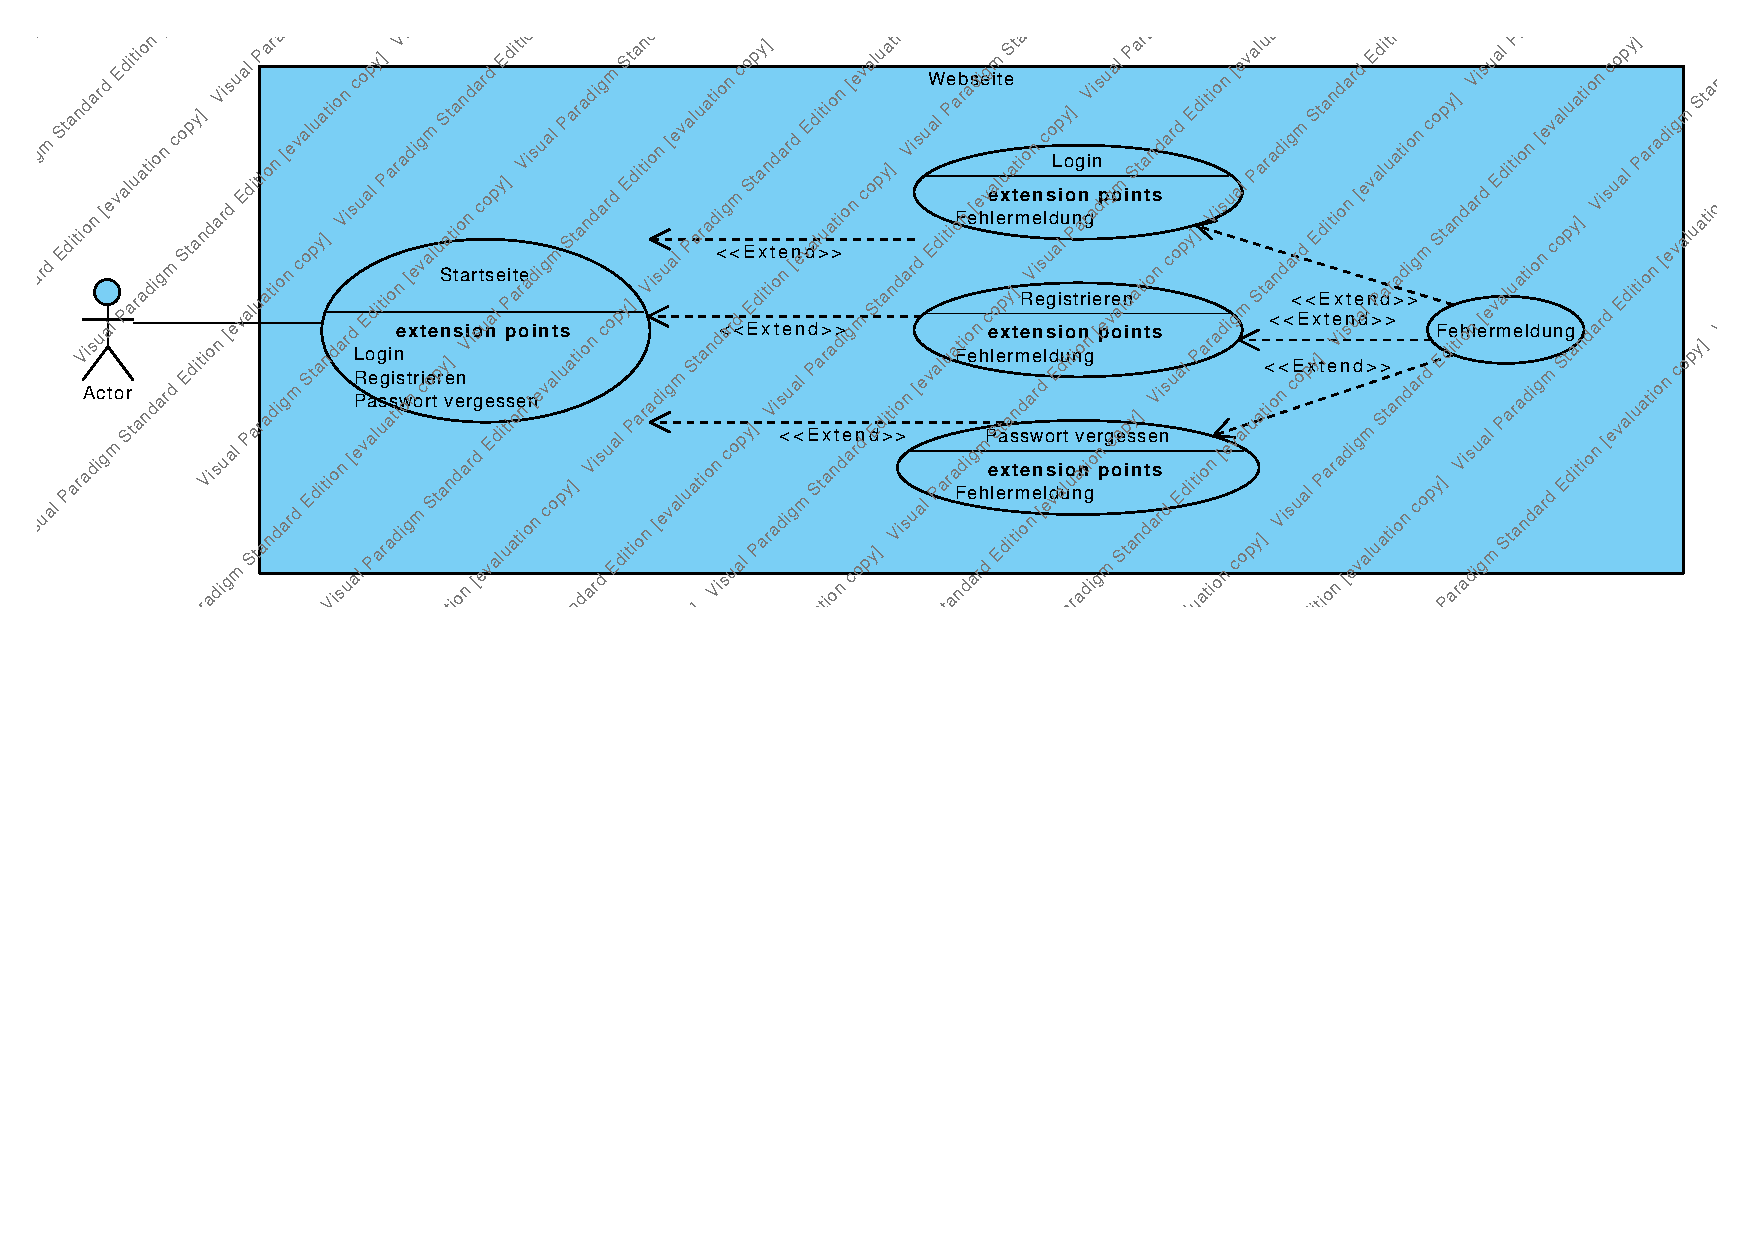
\includegraphics[width=\linewidth,]{gfx/webseite/startseite.pdf}
	\end{figure}
	\begin{tabular}{|l|p{.5\linewidth}|}
	\hline Use Case Nummer & 1.1 \\ 
	\hline Use Case Name & Startseite \\ 
	\hline Initiirender Akteur & Benutzer \\
	\hline Weitere Akteure &  \\
	\hline Kurzbeschreibung & der Benutzer ruft die Startseite im Browser auf und hat die M\"oglichkeit sich zu registrieren, einzuloggen und das Passwort neu anzufordern \\
	\hline Vorbedingung & nicht eingeloggt \\
	\hline Nachbedingung &  \\
	\hline \multicolumn{2}{|c|}{Funktionalitaet des UseCases}\\
	\hline Ablauf & Bentuzer ruft die Webseite auf \\
	\hline Alternativen &  \\
	\hline Ausnahmen &  \\
	\hline Benuzte Use Cases &  \\
	\hline \multicolumn{2}{|c|}{Weitere Inforamtionen} \\
	\hline Spezielle Anforderungen &  \\
	\hline Annahmen &  \\
	\hline
	\end{tabular} 
	\subsubsection{Login}
		\begin{tabular}{|l|p{.5\linewidth}|}
		\hline Use Case Nummer & 1.1.1 \\ 
		\hline Use Case Name & Login \\ 
		\hline Initiirender Akteur & Benutzer \\
		\hline Weitere Akteure & Admin \\
		\hline Kurzbeschreibung & Mit dem Login stehen die eigentlichen Funktionen im Browser zur Verf\"ugung \\
		\hline Vorbedingung & Benutzer ist registriert und nicht nicht eingeloggt \\
		\hline Nachbedingung & Benutzer ist eingeloggt \\
		\hline \multicolumn{2}{|c|}{Funktionalitaet des UseCases}\\
		\hline Ablauf & \begin{itemize}
			\item Der Benutzer gibt Email-Adresse und Passwort ein
			\item Der Benutzer klickt den Login Button
		\end{itemize} \\
		\hline Alternativen &  \\
		\hline Ausnahmen & \begin{itemize}
			\item Das Passwort ist falsch, es wird eine Fehlermeldung angezeigt und die Option Passwort vergessen angeboten
			\item Die Email-adresse ist noch nicht registriert, es wird eine Fehlermedldung angezeigt, und die Registrierung angeboten
		\end{itemize} \\
		\hline Benuzte Use Cases &  \\
		\hline \multicolumn{2}{|c|}{Weitere Inforamtionen} \\
		\hline Spezielle Anforderungen &  \\
		\hline Annahmen &  \\
		\hline
		\end{tabular}
			 
	\subsubsection{Registrieren}
		\begin{tabular}{|l|p{.5\linewidth}|}
		\hline Use Case Nummer & 1.1.2 \\ 
		\hline Use Case Name & Registrieren \\ 
		\hline Initiirender Akteur & Benutzer \\
		\hline Weitere Akteure &  \\
		\hline Kurzbeschreibung & Ein neuer Benutzer kann sich mit seiner Email-Adresse anmelden \\
		\hline Vorbedingung & Benutzer hat auf Registrieren geklickt \\
		\hline Nachbedingung & Benutzer ist eingeloggt \\
		\hline \multicolumn{2}{|c|}{Funktionalitaet des UseCases}\\
		\hline Ablauf & \begin{itemize}
			\item Benutzer gibt Email-Adresse und Passwort ein
			\item Benutzer w\"ahlt fakult\"at
			\item Benutzer klickt "jetzt mitmachen"
		\end{itemize} \\
		\hline Alternativen &  \\
		\hline Ausnahmen & \begin{itemize}
			\item Email-adresse ist schon vergeben, es wird eine Fehlermeldung angezeigt
			\item das Passwort ist zu kurz, es wird eine Fehlermeldung angezeit
			\item Keine Fakult\"at gewahlt, es wir eine Fehlermeldung angezeigt
		\end{itemize} \\
		\hline Benuzte Use Cases &  \\
		\hline \multicolumn{2}{|c|}{Weitere Inforamtionen} \\
		\hline Spezielle Anforderungen &  \\
		\hline Annahmen &  \\
		\hline
		\end{tabular} 
		
	\subsubsection{Passwort vergessen}
		\begin{tabular}{|l|p{.5\linewidth}|}
		\hline Use Case Nummer & 1.1.3 \\ 
		\hline Use Case Name & Passwort vergessen \\ 
		\hline Initiirender Akteur & Benutzer \\
		\hline Weitere Akteure &  \\
		\hline Kurzbeschreibung & Ein Benutzer hat die M\"oglichkeit sein Passwort neu anzufordern \\
		\hline Vorbedingung & Benutzer ist nicht eingeloggt \\
		\hline Nachbedingung & Benutzer hat eine Email bekommen \\
		\hline \multicolumn{2}{|c|}{Funktionalitaet des UseCases}\\
		\hline Ablauf & \begin{itemize}
			\item Benutzer gibt seine Email-Adresse an
			\item Benutzer klickt auf "jetzt Passwort anfordern"
		\end{itemize} \\
		\hline Alternativen &  \\
		\hline Ausnahmen & Email-Adresse ist nicht registriert, es wird eine Fehlermeldung angezeigt \\
		\hline Benuzte Use Cases &  \\
		\hline \multicolumn{2}{|c|}{Weitere Inforamtionen} \\
		\hline Spezielle Anforderungen &  \\
		\hline Annahmen &  \\
		\hline
		\end{tabular}
	\subsubsection{Fehlermeldung}
		\begin{tabular}{|l|p{.5\linewidth}|}
		\hline Use Case Nummer & 1.1.4 \\ 
		\hline Use Case Name & Fehlermeldung \\ 
		\hline Initiirender Akteur & Benutzer \\
		\hline Weitere Akteure &  \\
		\hline Kurzbeschreibung & Es wird dem Benutzer eine Fehlermeldung angezeigt und beleibt auf der aktuellen Seite \\
		\hline Vorbedingung &  \\
		\hline Nachbedingung & Fehlermeldung wir angezeigt \\
		\hline \multicolumn{2}{|c|}{Funktionalitaet des UseCases}\\
		\hline Ablauf & Fehlermeldung wird in die Aktuelle Seite eingebettet \\
		\hline Alternativen &  \\
		\hline Ausnahmen &  \\
		\hline Benuzte Use Cases &  \\
		\hline \multicolumn{2}{|c|}{Weitere Inforamtionen} \\
		\hline Spezielle Anforderungen &  \\
		\hline Annahmen &  \\
		\hline
		\end{tabular} 
<<<<<<< HEAD
	 

=======
%------------------
\subsection{Landingpage}

	\subsubsection{Landingpage}
	\begin{tabular}{|l|p{.5\linewidth}|}
	\hline Use Case Nummer & 1.2 \\ 
	\hline Use Case Name & Landingpage \\ 
	\hline Initiierender Akteur & Benutzer \\
	\hline Weitere Akteure & Admin \\
	\hline Kurzbeschreibung & Der Benutzer kann eine oder mehrere der verf\"ugbaren Aktivit\"aten ausw\"ahlen \\
	\hline Vorbedingung & Die Aktivit\"atenseite ist im Browser aufgerufen und die Liste von Aktivit\"aten wird angezeigt \\
	\hline Nachbedingung & Die Aktivit\"atenliste wird angezeigt, die ausgew\"ahlten Aktivit\"aten sind speziell hervorgehoben \\
	\hline \multicolumn{2}{|c|}{Funktionalitaet des UseCases}\\
	\hline Ablauf & \begin{itemize}
			\item 1. Benutzer w\"ahlt eine oder mehrere Aktivit\"aten aus
			\item 2. Die ausgew\"ahlten Aktivit\"aten werden als ausgew\"ahlt hervorgehoben
		\end{itemize} \\
	\hline Alternativen & - \\
	\hline Ausnahmen & Die Aktivit\"atenliste ist nicht verf\"ugbar \\
	\hline Benutzte Use Cases & 1.3.1 Aktivit\"aten ansehen \\
	\hline \multicolumn{2}{|c|}{Weitere Inforamtionen} \\
	\hline Spezielle Anforderungen & - \\
	\hline Annahmen & Der Benutzer w\"ahlt nur Aktivit\"aten aus, die noch nicht ausgew\"ahlt sind \\
	\hline
	\end{tabular}
%-----------------
\subsection{Aktivit\"aten}
>>>>>>> a66e7062aa58d82925d423a0aea5a264a3775ae3
	\subsubsection{Aktivit\"atenseite}
	\begin{tabular}{|l|p{.5\linewidth}|}
	\hline Use Case Nummer & 1.3 \\ 
	\hline Use Case Name & Aktivit\"atenseite \\ 
	\hline Initiierender Akteur & Benutzer \\
	\hline Weitere Akteure & Admin \\
	\hline Kurzbeschreibung & Der Benutzer kann eine Liste von verf\"ugbaren, ausgew\"ahlten und erledigten Aktivit\"aten ansehen, sowie Aktivit\"aten ausw\"ahlen, abw\"ahlen oder als erledigt markieren \\
	\hline Vorbedingung & Die Aktivit\"atenseite ist im Browser aufgerufen \\
	\hline Nachbedingung & Die Aktivit\"atenseite ist im Browser aufgerufen \\
	\hline \multicolumn{2}{|c|}{Funktionalitaet des UseCases}\\
	\hline Ablauf & 1. Benutzer ruft die Aktivit\"atenseite auf \\
	\hline Alternativen & - \\
	\hline Ausnahmen & Die Aktivit\"atenseite ist nicht verf\"ugbar \\
	\hline Benutzte Use Cases & - \\
	\hline \multicolumn{2}{|c|}{Weitere Inforamtionen} \\
	\hline Spezielle Anforderungen & - \\
	\hline Annahmen & - \\
	\hline
	\end{tabular} 
	\subsubsection{Aktivit\"aten ansehen}
	\begin{tabular}{|l|p{.5\linewidth}|}
	\hline Use Case Nummer & 1.3.1 \\ 
	\hline Use Case Name & Aktivit\"aten ansehen \\ 
	\hline Initiierender Akteur & Benutzer \\
	\hline Weitere Akteure & Admin \\
	\hline Kurzbeschreibung & Der Benutzer kann die auf der Seite dargestellte Liste von verf\"ugbaren Aktivit\"aten einsehen \\
	\hline Vorbedingung & Die Aktivit\"atenseite ist im Browser aufgerufen \\
	\hline Nachbedingung & Die Aktivit\"atenseite ist im Browser aufgerufen \\
	\hline \multicolumn{2}{|c|}{Funktionalitaet des UseCases}\\
	\hline Ablauf & 1. Der Benutzer sieht die Liste der Aktivit\"aten an \\
	\hline Alternativen & - \\
	\hline Ausnahmen & Die Aktivit\"atenliste ist nicht verf\"ugbar \\
	\hline Benutzte Use Cases & - \\
	\hline \multicolumn{2}{|c|}{Weitere Inforamtionen} \\
	\hline Spezielle Anforderungen & - \\
	\hline Annahmen & - \\
	\hline
	\end{tabular} 
	\subsubsection{Aktivit\"aten ausw\"ahlen}
	\begin{tabular}{|l|p{.5\linewidth}|}
	\hline Use Case Nummer & 1.3.2 \\ 
	\hline Use Case Name & Aktivit\"aten ausw\"ahlen \\ 
	\hline Initiierender Akteur & Benutzer \\
	\hline Weitere Akteure & Admin \\
	\hline Kurzbeschreibung & Der Benutzer kann eine oder mehrere der verf\"ugbaren Aktivit\"aten ausw\"ahlen \\
	\hline Vorbedingung & Die Aktivit\"atenseite ist im Browser aufgerufen und die Liste von Aktivit\"aten wird angezeigt \\
	\hline Nachbedingung & Die Aktivit\"atenliste wird angezeigt, die ausgew\"ahlten Aktivit\"aten sind speziell hervorgehoben \\
	\hline \multicolumn{2}{|c|}{Funktionalitaet des UseCases}\\
	\hline Ablauf & \begin{itemize}
			\item 1. Benutzer w\"ahlt eine oder mehrere Aktivit\"aten aus
			\item 2. Die ausgew\"ahlten Aktivit\"aten werden als ausgew\"ahlt hervorgehoben
		\end{itemize} \\
	\hline Alternativen & - \\
	\hline Ausnahmen & Die Aktivit\"atenliste ist nicht verf\"ugbar \\
	\hline Benutzte Use Cases & 1.3.1 Aktivit\"aten ansehen \\
	\hline \multicolumn{2}{|c|}{Weitere Inforamtionen} \\
	\hline Spezielle Anforderungen & - \\
	\hline Annahmen & Der Benutzer w\"ahlt nur Aktivit\"aten aus, die noch nicht ausgew\"ahlt sind \\
	\hline
	\end{tabular}
	\subsubsection{Aktivit\"aten als erledigt abhaken}
	\begin{tabular}{|l|p{.5\linewidth}|}
	\hline Use Case Nummer & 1.3.2.1 \\ 
	\hline Use Case Name & Aktivit\"aten als erledigt abhaken \\ 
	\hline Initiierender Akteur & Benutzer \\
	\hline Weitere Akteure & Admin \\
	\hline Kurzbeschreibung & Der Benutzer kann ausgew\"ahlte Aktivit\"aten, die er durchgef\"uhrt hat, als erledigt abhaken \\
	\hline Vorbedingung & Der Benutzer hat bereits eine oder mehrere Aktivit\"aten ausgew\"ahlt \\
	\hline Nachbedingung & Die abgehakte/n Aktivit\"at/en werden als solche markiert und dem Benutzer die entsprechende Punktzahl gutgeschrieben \\
	\hline \multicolumn{2}{|c|}{Funktionalitaet des UseCases}\\
	\hline Ablauf & \begin{itemize}
			\item 1. Benutzer hakt eine oder mehrere der ausgew\"ahlten Aktivit\"aten als erledigt ab
			\item 2. Die abgehakten Aktivit\"aten werden als erledigt markiert und dem Benutzer die entsprechenden Punkte gutgeschrieben
		\end{itemize} \\
	\hline Alternativen & - \\
	\hline Ausnahmen & Die Aktivit\"at ist in dem Zeitraum bzw. derzeit nicht verf\"ugbar \\
	\hline Benutzte Use Cases & 1.3.1 Aktivit\"aten ansehen \\
	\hline \multicolumn{2}{|c|}{Weitere Informationen} \\
	\hline Spezielle Anforderungen & - \\
	\hline Annahmen & - \\
	\hline
	\end{tabular} 
	\subsubsection{Aktivit\"aten abw\"ahlen}
	\begin{tabular}{|l|p{.5\linewidth}|}
	\hline Use Case Nummer & 1.3.2.2 \\ 
	\hline Use Case Name & Aktivit\"aten abw\"ahlen \\ 
	\hline Initiierender Akteur & Benutzer \\
	\hline Weitere Akteure & Admin \\
	\hline Kurzbeschreibung & Der Benutzer kann eine oder mehrere Aktivit\"aten, die er zuvor ausgew\"ahlt hat, wieder abw\"ahlen \\
	\hline Vorbedingung & Es wurden bereits Aktivit\"aten ausgew\"ahlt und diese werden als solche angezeigt \\
	\hline Nachbedingung & Die abgew\"ahlten Aktivit\"aten sind nicht mehr als ausgew\"ahlt markiert \\
	\hline \multicolumn{2}{|c|}{Funktionalitaet des UseCases}\\
	\hline Ablauf & \begin{itemize}
			\item 1. Benutzer w\"ahlt eine oder mehrere der ausgew\"ahlten Aktivit\"aten ab
			\item 2. Die abgew\"ahlten Aktivit\"aten werden nicht mehr als ausgew\"ahlt hervorgehoben
		\end{itemize} \\
	\hline Alternativen & - \\
	\hline Ausnahmen & Die Aktivit\"atenliste ist nicht verf\"ugbar \\
	\hline Benutzte Use Cases & Aktivit\"aten ansehen \\
	\hline \multicolumn{2}{|c|}{Weitere Inforamtionen} \\
	\hline Spezielle Anforderungen & - \\
	\hline Annahmen & - \\
	\hline
	\end{tabular} 
	\subsubsection{Aktivit\"aten bearbeiten}
	\begin{tabular}{|l|p{.5\linewidth}|}
	\hline Use Case Nummer & 1.3.3 \\ 
	\hline Use Case Name & Aktivit\"aten bearbeiten \\ 
	\hline Initiierender Akteur & Admin \\
	\hline Weitere Akteure & - \\
	\hline Kurzbeschreibung & Der Admin kann einzelne Aktivit\"aten bearbeiten (Name, Punktzahl, Zeitraum, etc.) \\
	\hline Vorbedingung & Die Aktivit\"atenseite ist im Browser aufgerufen und eine Aktivit\"at zur Bearbeitung ausgew\"ahlt \\
	\hline Nachbedingung & Die bearbeitete Aktivit\"at wird in ihrer neuen Form in der Aktivit\"atenliste angezeigt \\
	\hline \multicolumn{2}{|c|}{Funktionalitaet des UseCases}\\
	\hline Ablauf & \begin{itemize}
			\item 1. Der Admin w\"ahlt eine Aktivit\"at zur Bearbeitung aus
			\item 2. Der Admin speichert die Aktivit\"at mit den vorgenommenen \"Anderungen
		\end{itemize} \\
	\hline Alternativen & Der Admin l\"oscht die Aktivit\"at \\
	\hline Ausnahmen & Die Aktivit\"atenliste ist nicht verf\"ugbar \\
	\hline Benutzte Use Cases & 1.3.1 Aktivit\"aten ansehen \\
	\hline \multicolumn{2}{|c|}{Weitere Inforamtionen} \\
	\hline Spezielle Anforderungen & - \\
	\hline Annahmen & - \\
	\hline
	\end{tabular} 
\subsection{Energiespavorschl\"age}
%---------------------------------------------
\subsection{Rangliste}
	\begin{figure}[h]
		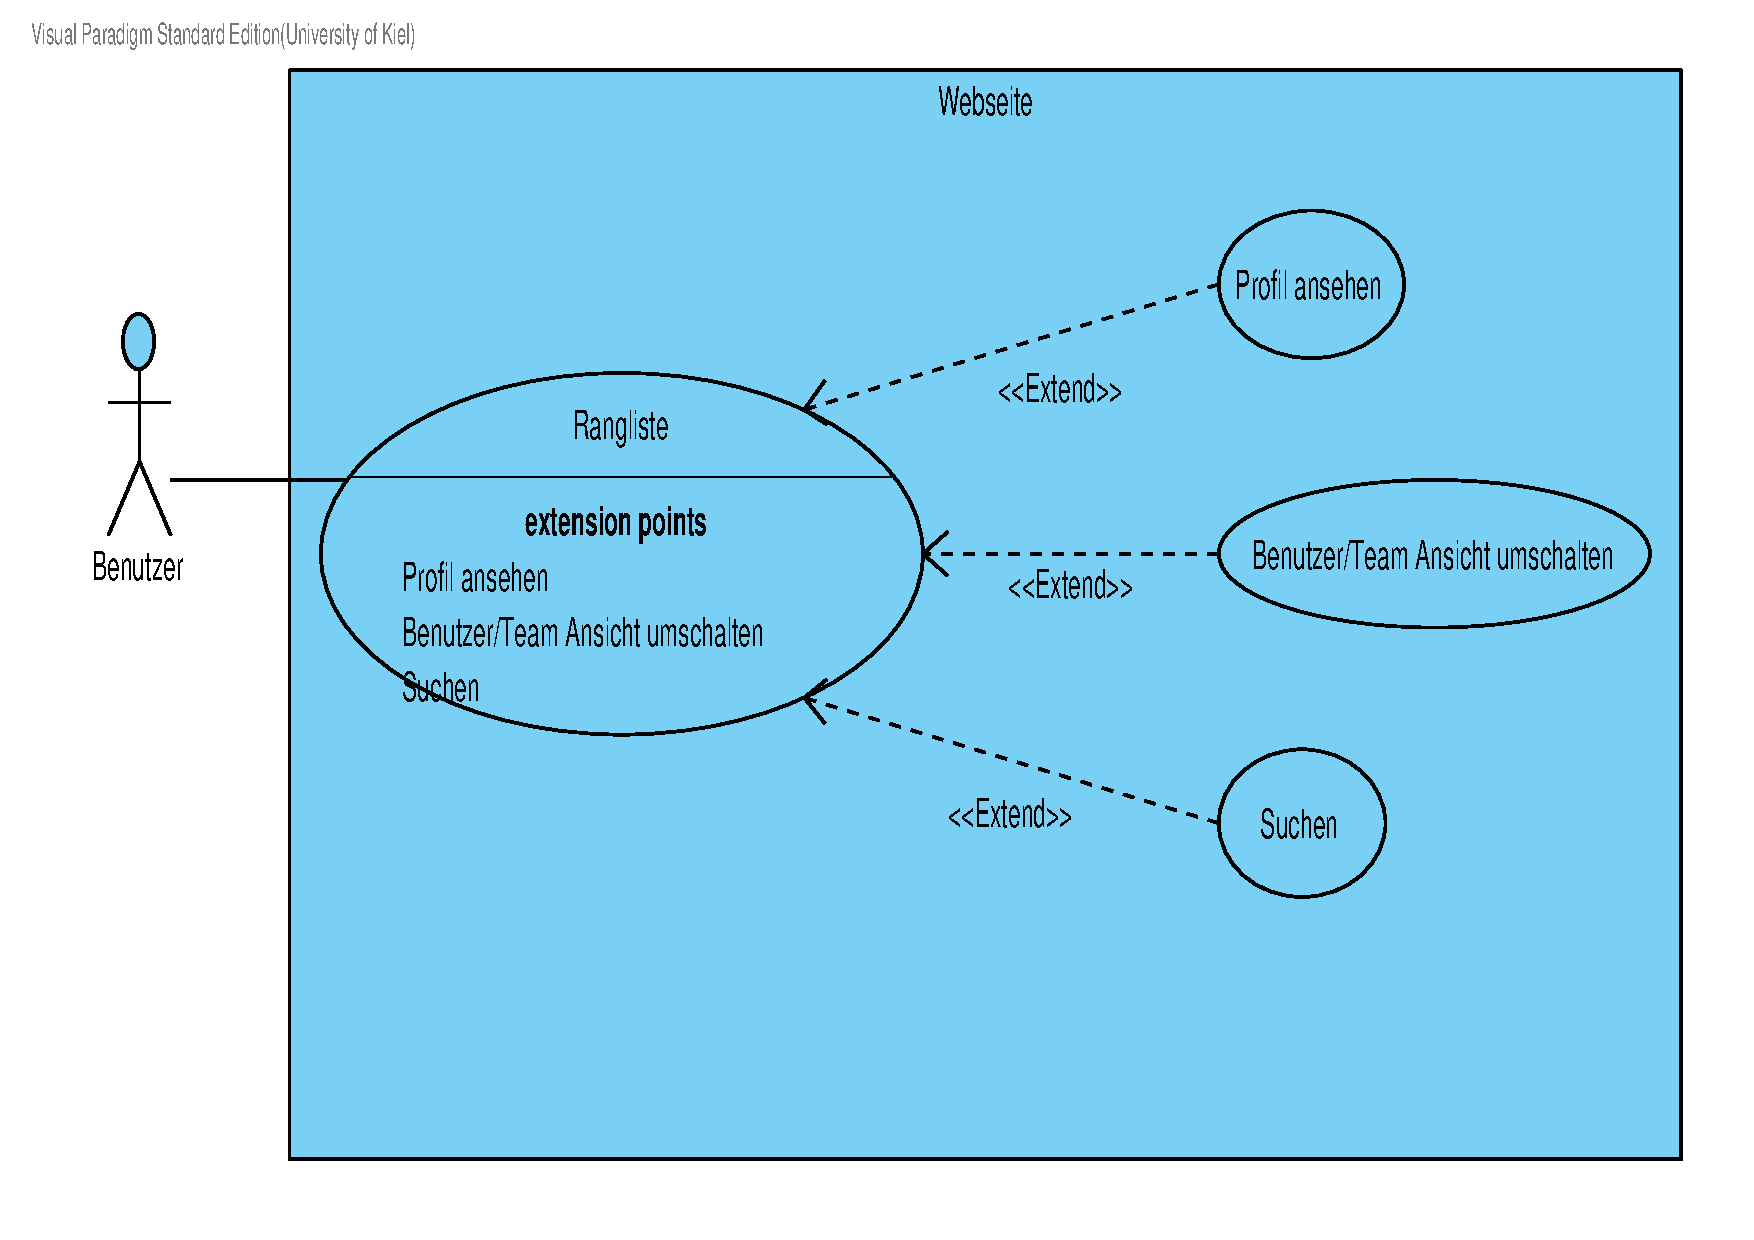
\includegraphics[width=\linewidth,]{gfx/webseite/rangliste.pdf}
	\end{figure}
	\subsubsection{Rangliste Ansehen}
		\begin{tabular}{|l|p{.5\linewidth}|}
		\hline Use Case Nummer & 1.5 \\ 
		\hline Use Case Name & Rangliste Ansehen \\ 
		\hline Initiirender Akteur & Benutzer \\
		\hline Weitere Akteure &  \\
		\hline Kurzbeschreibung & Der Benutzer kann die Rangliste ansehen \\
		\hline Vorbedingung & Der Benutzer ist eingeloggt \\
		\hline Nachbedingung &  \\
		\hline \multicolumn{2}{|c|}{Funktionalitaet des UseCases}\\
		\hline Ablauf & Der Benutzer kann die Rangliste ansehen \\
		\hline Alternativen & Der Benutzer kann Suchen \\
		\hline Ausnahmen &  \\
		\hline Benuzte Use Cases &  \\
		\hline \multicolumn{2}{|c|}{Weitere Inforamtionen} \\
		\hline Spezielle Anforderungen &  \\
		\hline Annahmen &  \\
		\hline
		\end{tabular}
	\subsubsection{Profil ansehen}
		\begin{tabular}{|l|p{.5\linewidth}|}
		\hline Use Case Nummer & 1.5.1 \\ 
		\hline Use Case Name & Profil ansehen \\ 
		\hline Initiirender Akteur & Benutzer \\
		\hline Weitere Akteure &  \\
		\hline Kurzbeschreibung & Eine Ansicht eines Profils von einem Team oder einem Benutzer \\
		\hline Vorbedingung & Es wurde ein Profil angeklickt \\
		\hline Nachbedingung & Das Profil wird angezeigt \\
		\hline \multicolumn{2}{|c|}{Funktionalitaet des UseCases}\\
		\hline Ablauf & \begin{itemize}
			\item Benuzter klickt auf ein Profil
			\item Benutzer wird Profil angezeigt
		\end{itemize} \\
		\hline Alternativen &  \\
		\hline Ausnahmen &  \\
		\hline Benuzte Use Cases &  \\
		\hline \multicolumn{2}{|c|}{Weitere Inforamtionen} \\
		\hline Spezielle Anforderungen &  \\
		\hline Annahmen &  \\
		\hline
		\end{tabular}
	\subsubsection{Benutzer/Team Ansicht wechseln}
		\begin{tabular}{|l|p{.5\linewidth}|}
		\hline Use Case Nummer & 1.5.2 \\ 
		\hline Use Case Name & Benutzer/Team Ansicht wechseln \\ 
		\hline Initiirender Akteur & Benutzer \\
		\hline Weitere Akteure &  \\
		\hline Kurzbeschreibung & Der Benutzer kann zwischen der Benutzer Rangliste und der Team Rangliste hin und her schalten \\
		\hline Vorbedingung & Rangliste wird angezeigt \\
		\hline Nachbedingung & Ansicht wurde umgeschaltet \\
		\hline \multicolumn{2}{|c|}{Funktionalitaet des UseCases}\\
		\hline Ablauf & \begin{itemize}
			\item Benutzer klickt auf "Team"
			\item Team Ansicht wird angezeigt
		\end{itemize} \\
		\hline Alternativen & \begin{itemize}
					\item Benutzer klickt auf "Benutzer"
					\item Benutzer Ansicht wird angezeigt
				\end{itemize} \\
		\hline Ausnahmen &  \\
		\hline Benuzte Use Cases &  \\
		\hline \multicolumn{2}{|c|}{Weitere Inforamtionen} \\
		\hline Spezielle Anforderungen &  \\
		\hline Annahmen &  \\
		\hline
		\end{tabular}
		
		\subsubsection{Suche}
				\begin{tabular}{|l|p{.5\linewidth}|}
				\hline Use Case Nummer & 1.5.3 \\ 
				\hline Use Case Name & Suche \\ 
				\hline Initiirender Akteur & Benutzer \\
				\hline Weitere Akteure &  \\
				\hline Kurzbeschreibung & Der Benutzer kann nach Teams und Benutzern suchen \\
				\hline Vorbedingung &  \\
				\hline Nachbedingung & Suchergebnisse werden angezeigt \\
				\hline \multicolumn{2}{|c|}{Funktionalitaet des UseCases}\\
				\hline Ablauf & \begin{itemize}
					\item Benutzer gibt Suchanfrage ein
					\item Benutzer klickt suchen
					\item Suchergebnisse werden angezeigt
				\end{itemize} \\
				\hline Alternativen &  \\
				\hline Ausnahmen & Wenn keine Ergebnisse gefunden werden wird dies angezeigt \\
				\hline Benuzte Use Cases &  \\
				\hline \multicolumn{2}{|c|}{Weitere Inforamtionen} \\
				\hline Spezielle Anforderungen &  \\
				\hline Annahmen &  \\
				\hline
				\end{tabular}
%-----------------------------
\subsection{Statistiken}
%-----------------------------
\subsection{AdminBereich}
%-----------------------------
\subsection{Profilseite}
	\subsubsection{Profilseite \"andern}
		\begin{tabular}{|l|p{.5\linewidth}|}
		\hline Use Case Nummer & 1.8 \\ 
		\hline Use Case Name & Profilseite \"andern \\ 
		\hline Initiirender Akteur & Benutzer \\
		\hline Weitere Akteure & Admin \\
		\hline Kurzbeschreibung & Der Benutzer kann verschiedene Informationen seines Profils bearbeiten, wie Profilbild, Passwort, Benachrichtigungseinstellungen oder Fakultät und besitzt die Möglichkeit sein Profil zu löschen \\
		\hline Vorbedingung & Die Profilseite ist im Browser aufgerufen \\
		\hline Nachbedingung & Die Profilseite wird mit den vorgenommenen \"Anderungen angezeigt oder ist gel\"oscht worden \\
		\hline \multicolumn{2}{|c|}{Funktionalitaet des UseCases}\\
		\hline Ablauf & \begin{itemize}
					\item 1. Der Benutzer w\"ahlt eine Information, die er bearbeiten m\"ochte aus und bearbeitet diese
					\item 2. Der Benutzer speichert die ge\"anderten Informationen und diese werden ins System \"ubernommen
				\end{itemize}\\
		\hline Alternativen & - \\
		\hline Ausnahmen & - \\
		\hline Benuzte Use Cases & - \\
		\hline \multicolumn{2}{|c|}{Weitere Informationen} \\
		\hline Spezielle Anforderungen &  \\
		\hline Annahmen &  \\
		\hline
		\end{tabular}
		
			\subsubsection{Profil sperren}
		\begin{tabular}{|l|p{.5\linewidth}|}
		\hline Use Case Nummer & 1.8.1 \\ 
		\hline Use Case Name & Profil sperren \\ 
		\hline Initiirender Akteur & Admin \\
		\hline Weitere Akteure & - \\
		\hline Kurzbeschreibung & Der Admin kann ein Profil sperren, wenn irgendeine Form von Missverhalten vorliegt \\
		\hline Vorbedingung & Die Profilseite ist im Browser aufgerufen \\
		\hline Nachbedingung & Die Profilseite wird dem Admin als gesperrt angezeigt \\
		\hline \multicolumn{2}{|c|}{Funktionalitaet des UseCases}\\
		\hline Ablauf & \begin{itemize}
					\item 1. Der Admin \"offnet die Profilseite des zu sperrenden Profils
					\item 2. Der Admin sperrt das entsprechende Profil, welches im Anschluss f\"ur Benutzer nicht mehr sichtbar und verwendbar ist
				\end{itemize}\\
		\hline Alternativen & - \\
		\hline Ausnahmen & - \\
		\hline Benuzte Use Cases & - \\
		\hline \multicolumn{2}{|c|}{Weitere Informationen} \\
		\hline Spezielle Anforderungen &  \\
		\hline Annahmen &  \\
		\hline
		\end{tabular}
		
			\subsubsection{Profil reaktivieren}
		\begin{tabular}{|l|p{.5\linewidth}|}
		\hline Use Case Nummer & 1.8.1.1 \\ 
		\hline Use Case Name & Profil reaktivieren \\ 
		\hline Initiierender Akteur & Admin \\
		\hline Weitere Akteure & - \\
		\hline Kurzbeschreibung & Admin kann ein zuvor gesperrtes Profil reaktivieren \\
		\hline Vorbedingung & Die gesperrte Profilseite ist im Browser aufgerufen \\
		\hline Nachbedingung & Die Profilseite ist wieder sichtbar \\
		\hline \multicolumn{2}{|c|}{Funktionalitaet des UseCases}\\
		\hline Ablauf & \begin{itemize}
					\item 1. Der Admin ruft ein gesperrtes Profil auf
					\item 2. Der Admin reaktiviert das Profil, sodass es f\"ur alle Benutzer wieder sichtbar ist und der Profilinhaber wieder alle Funktionen nutzen kann
				\end{itemize}\\
		\hline Alternativen & - \\
		\hline Ausnahmen & - \\
		\hline Benuzte Use Cases & - \\
		\hline \multicolumn{2}{|c|}{Weitere Informationen} \\
		\hline Spezielle Anforderungen &  \\
		\hline Annahmen &  \\
		\hline
		\end{tabular}
		
			\subsubsection{Profilinhaber zum Admin bef\"ordern}
		\begin{tabular}{|l|p{.5\linewidth}|}
		\hline Use Case Nummer & 1.8.2 \\ 
		\hline Use Case Name & Profilinhaber zum Admin bef\"ordern \\ 
		\hline Initiirender Akteur & Admin \\
		\hline Weitere Akteure & Benutzer, der zum Admin wird \\
		\hline Kurzbeschreibung & Ein Admin kann einen Benutzer zum Admin ernennen und ihm so Administratorzugriff gew\"ahren \\
		\hline Vorbedingung & Die Profilseite ist im Browser aufgerufen \\
		\hline Nachbedingung & Die Profilseite wird im Browser angezeigt und der Benutzer ist im System als Admin registriert \\
		\hline \multicolumn{2}{|c|}{Funktionalitaet des UseCases}\\
		\hline  Ablauf & \begin{itemize}
					\item 1. Der Admin w\"ahlt das Profil des Benutzers aus, den er zum Admin bef\"ordern m\"ochte
					\item 2. Der Admin bef\"ordert den Benutzer \"uber einen Men\"upunkt zum Administrator
				\end{itemize}\\
		\hline Alternativen & - \\
		\hline Ausnahmen & - \\
		\hline Benuzte Use Cases & - \\
		\hline \multicolumn{2}{|c|}{Weitere Informationen} \\
		\hline Spezielle Anforderungen &  \\
		\hline Annahmen & Das Profil des zu bef\"ordernden Benutzers ist nicht gesperrt \\
		\hline
		\end{tabular}
		
			\subsubsection{Profil l\"oschen}
		\begin{tabular}{|l|p{.5\linewidth}|}
		\hline Use Case Nummer & 1.8.3 \\ 
		\hline Use Case Name & Profil l\"oschen \\ 
		\hline Initiirender Akteur & Admin \\
		\hline Weitere Akteure & - \\
		\hline Kurzbeschreibung & Der Admin kann ausgew\"ahlte Profile l\"oschen \\
		\hline Vorbedingung & Die Profilseite ist im Browser aufgerufen \\
		\hline Nachbedingung & Das Profil ist aus dem System gel\"oscht \\
		\hline \multicolumn{2}{|c|}{Funktionalitaet des UseCases}\\
		\hline  Ablauf & \begin{itemize}
					\item 1. Der Admin w\"ahlt das zu löschende Profil aus
					\item 2. Der Admin l\"oscht das Profil
				\end{itemize}\\
		\hline Alternativen & - \\
		\hline Ausnahmen & - \\
		\hline Benuzte Use Cases & - \\
		\hline \multicolumn{2}{|c|}{Weitere Informationen} \\
		\hline Spezielle Anforderungen & - \\
		\hline Annahmen & - \\
		\hline
		\end{tabular}
%-----------------------------
\subsection{Andoid App}
\begin{figure}[h]
		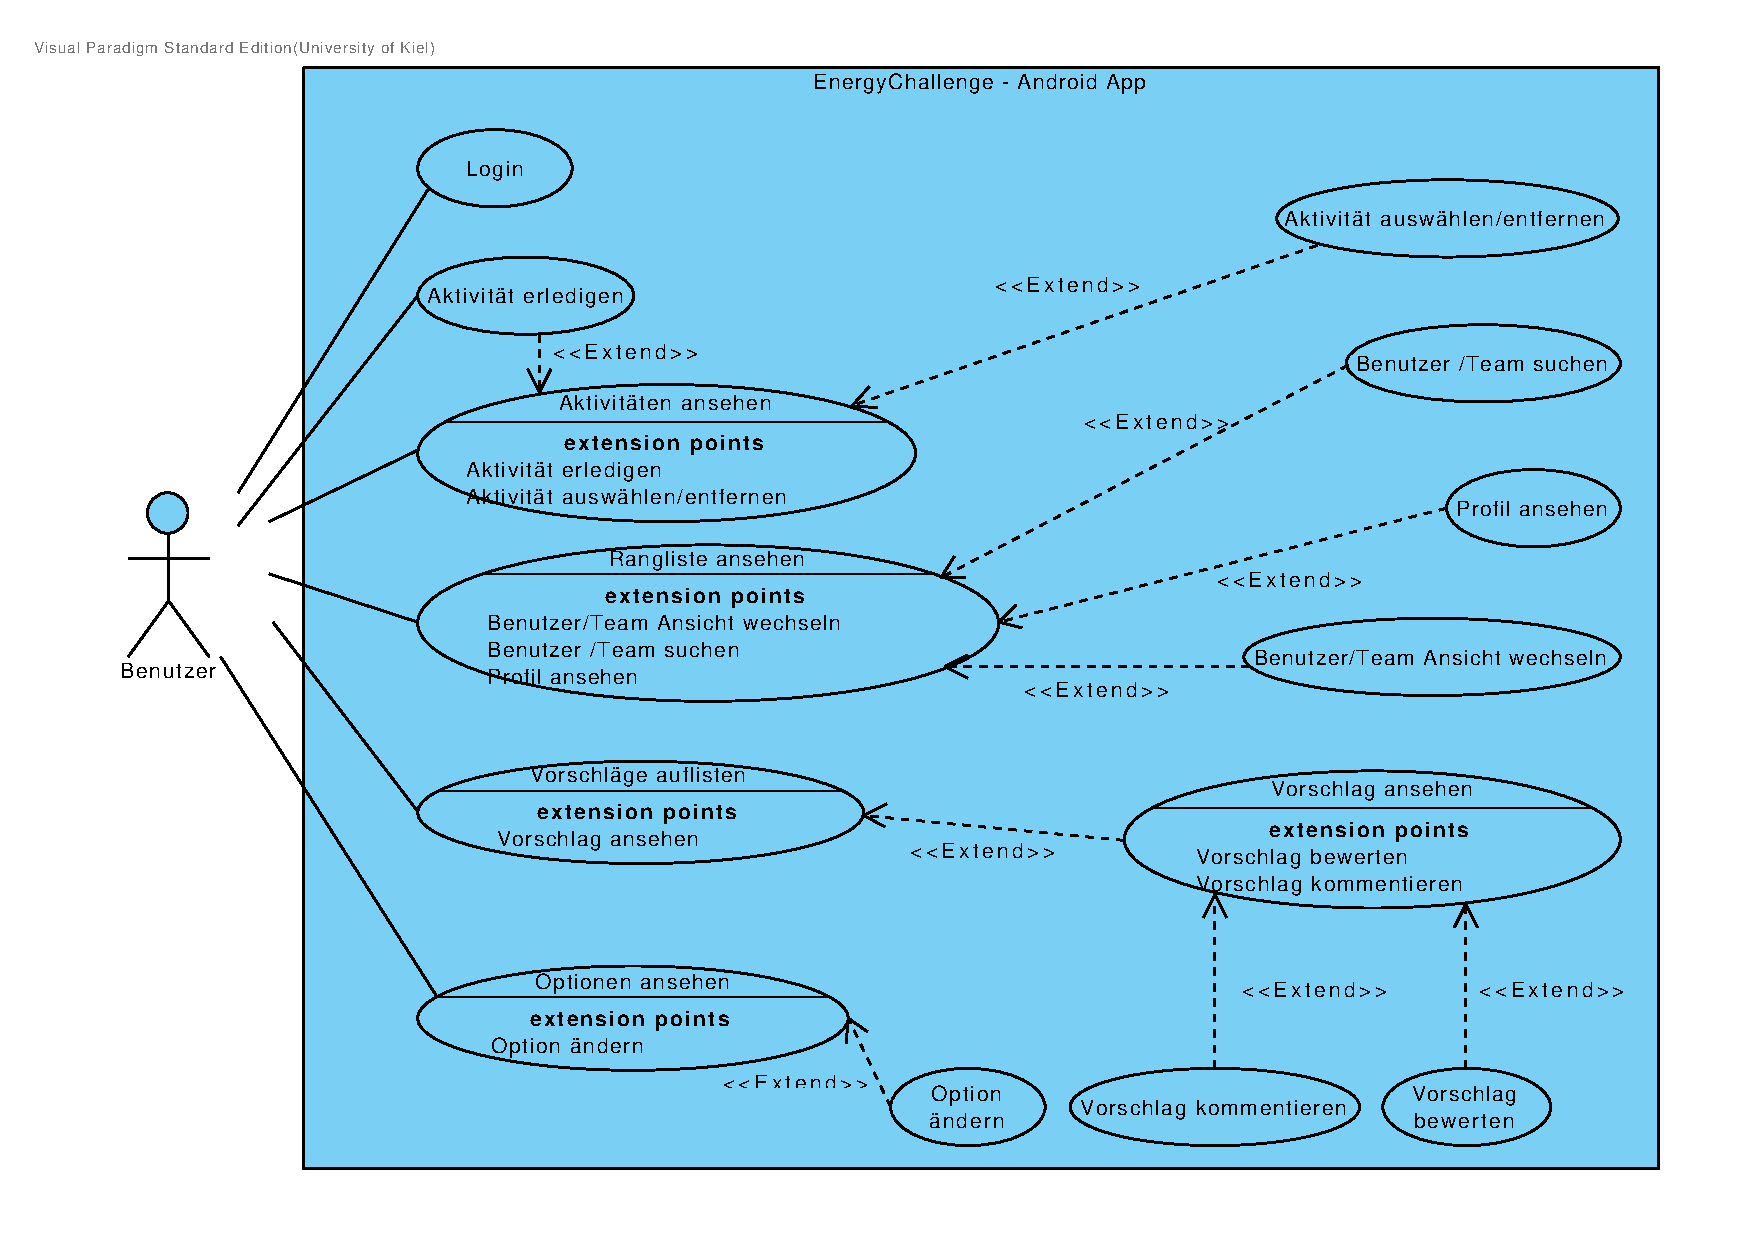
\includegraphics[width=\linewidth,]{gfx/androidapp/overview.pdf}
	\end{figure}
\subsubsection{Login}
		\begin{tabular}{|l|p{.5\linewidth}|}
		\hline Use Case Nummer & 2.1 \\ 
		\hline Use Case Name & Login \\ 
		\hline Initiirender Akteur & Benutzer \\
		\hline Weitere Akteure &  \\
		\hline Kurzbeschreibung & Der Benutzer muss sich einmalig anmelden um die App zu nutzen \\
		\hline Vorbedingung & Benutzer hat sich noch nie in der App angemeldet \\
		\hline Nachbedingung & Der Benutzer hat zugriff auf die Funktionen der App \\
		\hline \multicolumn{2}{|c|}{Funktionalitaet des UseCases}\\
		\hline Ablauf & \begin{itemize}
			\item der Benutzer started die App und muss zun\"acht Email-Adresse und Passwort eingeben
			\item der Benutzer klickt auf einloggen
		\end{itemize} \\
		\hline Alternativen &  \\
		\hline Ausnahmen & Bei Falschen Login-Daten wird auf die Webseite verwiesen \\
		\hline Benuzte Use Cases &  \\
		\hline \multicolumn{2}{|c|}{Weitere Inforamtionen} \\
		\hline Spezielle Anforderungen &  \\
		\hline Annahmen & Benutzer hat sich auf der Webseite angemeldet \\
		\hline
		\end{tabular}
\subsubsection{Aktivit\"at erledigen}
		\begin{tabular}{|l|p{.5\linewidth}|}
		\hline Use Case Nummer & 2.2 \\ 
		\hline Use Case Name & Aktivit\"at erledigen \\ 
		\hline Initiirender Akteur & Benutzer \\
		\hline Weitere Akteure &  \\
		\hline Kurzbeschreibung & Der Benutzer kann von der App direckt ausgew\"ahlte Aktivit\"aten erledigen \\
		\hline Vorbedingung & Benutzer ist eingeloggt \\
		\hline Nachbedingung & Benutzer hat Aktivit\"at ausgef\"uhrt \\
		\hline \multicolumn{2}{|c|}{Funktionalitaet des UseCases}\\
		\hline Ablauf & \begin{itemize}
			\item Benutzer klickt auf eine Aktivit\"at
			\item Benutzer best\"atigt die Aktivit\"at
		\end{itemize} \\
		\hline Alternativen &  \\
		\hline Ausnahmen &  \\
		\hline Benuzte Use Cases &  \\
		\hline \multicolumn{2}{|c|}{Weitere Inforamtionen} \\
		\hline Spezielle Anforderungen &  \\
		\hline Annahmen &  \\
		\hline
		\end{tabular}

\subsubsection{Aktivit\"aten ansehen}
		\begin{tabular}{|l|p{.5\linewidth}|}
		\hline Use Case Nummer & 2.3 \\ 
		\hline Use Case Name & Aktivi\"aten ansehn \\ 
		\hline Initiirender Akteur & Benutzer \\
		\hline Weitere Akteure &  \\
		\hline Kurzbeschreibung & Benutzer kann die ausgew\"ahlten Aktivit\"aten hinzuf\"ugen und entfernen \\
		\hline Vorbedingung & Benutzer ist eingeloggt \\
		\hline Nachbedingung & Benutzer sieht Aktivit\"aten \\
		\hline \multicolumn{2}{|c|}{Funktionalitaet des UseCases}\\
		\hline Ablauf & \begin{itemize}
			\item Benutzer navigiert im Menu zu "Aktivit\"aten"
			\item Benutzer werden Aktivit\"aten angezeigt
		\end{itemize} \\
		\hline Alternativen &  \\
		\hline Ausnahmen &  \\
		\hline Benuzte Use Cases &  \\
		\hline \multicolumn{2}{|c|}{Weitere Inforamtionen} \\
		\hline Spezielle Anforderungen &  \\
		\hline Annahmen &  \\
		\hline
		\end{tabular}

\subsubsection{Aktivit\"at ausw\"ahlen}
		\begin{tabular}{|l|p{.5\linewidth}|}
		\hline Use Case Nummer & 2.3.1 \\ 
		\hline Use Case Name & Aktivit\"at ausw\"ahlen \\ 
		\hline Initiirender Akteur & Benutzer \\
		\hline Weitere Akteure &  \\
		\hline Kurzbeschreibung & Benutzer f\"ugt eine Aktivit\"at zu seinen Ausgew\"ahlten hinzu und kann sie auch entfernen \\
		\hline Vorbedingung &  \\
		\hline Nachbedingung &  \\
		\hline \multicolumn{2}{|c|}{Funktionalitaet des UseCases}\\
		\hline Ablauf & \begin{itemize}
			\item Benutzer klickt auf "hinzuf\"ugen"
			\item Aktivit\"at wir den Ausgew\"ahlten hinzugef\"ugt
		\end{itemize} \\
		\hline Alternativen & \begin{itemize}
			\item Benutzer klickt auf "Entfernen"
			\item Aktivit\"at wird aus den Ausgew\"ahlten entfernt
		\end{itemize}  \\
		\hline Ausnahmen &  \\
		\hline Benuzte Use Cases &  \\
		\hline \multicolumn{2}{|c|}{Weitere Inforamtionen} \\
		\hline Spezielle Anforderungen &  \\
		\hline Annahmen & Benutzer ist eingeloggt \\
		\hline
		\end{tabular}

\subsubsection{Rangliste ansehen}
		\begin{tabular}{|l|p{.5\linewidth}|}
		\hline Use Case Nummer & 2.4 \\ 
		\hline Use Case Name & Rangliste ansehen\\ 
		\hline Initiirender Akteur & Benutzer \\
		\hline Weitere Akteure &  \\
		\hline Kurzbeschreibung & Benutzer kann die Aktuelle Rangliste der Benutzer und Teams ansehen \\
		\hline Vorbedingung & Benutzer ist eingeloggt \\
		\hline Nachbedingung & Rangliste wird angezeigt \\
		\hline \multicolumn{2}{|c|}{Funktionalitaet des UseCases}\\
		\hline Ablauf & \begin{itemize}
			\item Benutzer w\"ahlt im Menu "Rangliste"
			\item die Rangliste wird angezeigt
		\end{itemize} \\
		\hline Alternativen &  \\
		\hline Ausnahmen &  \\
		\hline Benuzte Use Cases &  \\
		\hline \multicolumn{2}{|c|}{Weitere Inforamtionen} \\
		\hline Spezielle Anforderungen &  \\
		\hline Annahmen &  \\
		\hline
		\end{tabular}

\subsubsection{Ansicht \"andern}
		\begin{tabular}{|l|p{.5\linewidth}|}
		\hline Use Case Nummer & 2.4.1 \\ 
		\hline Use Case Name & Ansicht \"andern \\ 
		\hline Initiirender Akteur & Benutzer \\
		\hline Weitere Akteure &  \\
		\hline Kurzbeschreibung & Der Benutzer kann zwischen der Benutzer- und der Team-Ranglisten-Ansicht wechseln \\
		\hline Vorbedingung & Benutzer ist in Ranglisten Ansicht \\
		\hline Nachbedingung & Benutzer ist in der Jeweils anderen Ranglisten Ansicht \\
		\hline \multicolumn{2}{|c|}{Funktionalitaet des UseCases}\\
		\hline Ablauf & \begin{itemize}
			\item Benutzer wischt \"uber den Bildschirm
			\item Die Ansicht wechselt
		\end{itemize} \\
		\hline Alternativen &  \\
		\hline Ausnahmen &  \\
		\hline Benuzte Use Cases &  \\
		\hline \multicolumn{2}{|c|}{Weitere Inforamtionen} \\
		\hline Spezielle Anforderungen &  \\
		\hline Annahmen &  \\
		\hline
		\end{tabular}
		

\subsubsection{Profil ansehen}
		\begin{tabular}{|l|p{.5\linewidth}|}
		\hline Use Case Nummer & 2.4.2 \\ 
		\hline Use Case Name & Profil ansehen \\ 
		\hline Initiirender Akteur & Benutzer \\
		\hline Weitere Akteure &  \\
		\hline Kurzbeschreibung & Der Benutzer kann die Profile von Benutzern und Team ansehen \\
		\hline Vorbedingung & Benutzer hat auf ein Benutzer oder Team geklickt \\
		\hline Nachbedingung & Benutzer sieht Profil \\
		\hline \multicolumn{2}{|c|}{Funktionalitaet des UseCases}\\
		\hline Ablauf & \begin{itemize}
			\item Benutzer klickt auf ein Benutzer oder Team
			\item Das Profil des Entspechenden Benutzers oder Teams wird dargestellt
		\end{itemize} \\
		\hline Alternativen &  \\
		\hline Ausnahmen &  \\
		\hline Benuzte Use Cases &  \\
		\hline \multicolumn{2}{|c|}{Weitere Inforamtionen} \\
		\hline Spezielle Anforderungen &  \\
		\hline Annahmen &  \\
		\hline
		\end{tabular}

\subsubsection{Suche}
		\begin{tabular}{|l|p{.5\linewidth}|}
		\hline Use Case Nummer & 2.4.3 \\ 
		\hline Use Case Name & Suche \\ 
		\hline Initiirender Akteur & Benutzer \\
		\hline Weitere Akteure &  \\
		\hline Kurzbeschreibung & Benutzer kann nach anderen Benutzern und Teams suchen \\
		\hline Vorbedingung &  \\
		\hline Nachbedingung & Benutzer werden die Suchergebnisse angezeigt \\
		\hline \multicolumn{2}{|c|}{Funktionalitaet des UseCases}\\
		\hline Ablauf & \begin{itemize}
			\item Benutzer gibt Suchbegriff ein.
			\item Benutzer klickt auf suchen
			\item Benutzer werden Suchergebnisse angezeigt
		\end{itemize} \\
		\hline Alternativen & Wurden keine Treffer gefunden, so wird das angezeigt \\
		\hline Ausnahmen &  \\
		\hline Benuzte Use Cases &  \\
		\hline \multicolumn{2}{|c|}{Weitere Inforamtionen} \\
		\hline Spezielle Anforderungen &  \\
		\hline Annahmen &  \\
		\hline
		\end{tabular}
%TODO List PROPOSAL,..
%TODO USER menu
%TODO Muster:
\subsubsection{title}
		\begin{tabular}{|l|p{.5\linewidth}|}
		\hline Use Case Nummer &  \\ 
		\hline Use Case Name &  \\ 
		\hline Initiirender Akteur &  \\
		\hline Weitere Akteure &  \\
		\hline Kurzbeschreibung &  \\
		\hline Vorbedingung &  \\
		\hline Nachbedingung &  \\
		\hline \multicolumn{2}{|c|}{Funktionalitaet des UseCases}\\
		\hline Ablauf &  \\
		\hline Alternativen &  \\
		\hline Ausnahmen &  \\
		\hline Benuzte Use Cases &  \\
		\hline \multicolumn{2}{|c|}{Weitere Inforamtionen} \\
		\hline Spezielle Anforderungen &  \\
		\hline Annahmen &  \\
		\hline
		\end{tabular}

%------------------------------------------------
% Produktdaten
%------------------------------------------------
\section{Produktdaten}
Die Daten werden in einer Datenbank gespeichert \\
\begin{itemize}
\item Benutzerdaten: 
\begin{itemize}
\item Vorname
\item Name
\item E-Mail Adresse
\item Passwort (verschlüsselt)
\item Foto
\item Institut
\item Rolle (Benutzer, Administrator)
\item Teamname
\item ausgewählte Aktivitäten
\item erledigte Aktivitäten
\item Punktzahl
\item laufende Challenges
\item abgeschlossene Challenges
\end{itemize}

\item Aktivitäten: 
\begin{itemize}
\item Aktivitätsname
\item Häufigkeitsattribut (täglich, wöchentlich, etc.)
\item Punkte für Aktivität
\item Challengenamen
\item Challengezeitraum
\item Challengepunkte
\end{itemize}

\item Vorschläge:
\begin{itemize}
\item Vorschlagsname
\item vorgeschlagene Punktzahl
\item Vorschlagserläuterung (wenn aus Name nicht ersichtlich)
\item Kommentare
\item Bewertungen
\end{itemize}

\item Statistik:
\begin{itemize}
\item Besucherzahl (Anzahl Logins)
\item Besucherzahl (Anzahl Startseitenzugriffe)
\end{itemize}
\end{itemize}







%------------------------------------------------
% Produktleistung
%------------------------------------------------
\section{Produktleistungen}

\subsection{L100/Client} 
Das System unterstützt die Anmeldung mehrerer Benutzer mit mehreren Clients (Webseite und/oder App) an einen zentralen Server. Der Client beinhaltet die Möglichkeit, Befehle vom Nutzer anzunehmen und sie an den Server weiterzuleiten. 

\subsection{L110/Antwortzeit} 
Nutzeranfragen werden in wenigen Sekunden bearbeitet, damit ein schnelle Nutzung ermöglicht wird. Im Falle, dass zwischen Client und Server Objekte, wie Fotos zum Upload, verschickt werden, kann die Antwortzeit minimal ansteigen. 

\subsection{L110/Ladezeit} 
Die Webseite benötigt nur eine kurze Zeit zum Starten. Diese ist natürlich von äußeren Faktoren (benutzter PC, Internetverbindung, etc.) abhängig. 

\subsection{L200/Server} 
Das System hat einen zentralen Server. Der Server bietet den Zugriff auf die Webseite und die die App an. 

\subsection{L300/Datenbank} 
Das System besitzt eine integrierte Datenbank. In der Datenbank werden alle relevanten Daten zum Betrieb der Webseite und der App gespeichert. Dies sind die Aktivitäten, Profile, Statistiken, Team-/Benutzerlisten, Ranglisten und Vorschläge, sowie Kommentare und Bewertungen.

\subsection{L310/Statistik} 
Die Datenbank erstellt Statistiken über die Besucherzahlen, die Anzahl aller erledigten Aktivitäten, die Anzahl aller gesammelten Punkte und die beliebtesten Aktivitäten. Des Weiteren wird mit der Datenbank eine Rangliste der Benutzer mit den meisten Punkten erstellt.

\subsection{L400/Benutzersicherheit} 
Die Webseiten- und die Appoberfläche sind so aufgebaut, dass der Benutzer keine unbeabsichtigten Eingaben tätigen kann, ohne, dass nachgefragt wird, ob er diese tätigen möchte. Nur ein Systemadministrator kann die Webseite und die App vom Server entfernen oder hinzufügen.


%------------------------------------------------
% Benutzeroberflache
%------------------------------------------------
\section{Benutzeroberfl\"ache}
\subsection{Webseite}
\subsection{Android App}
%------------------------------------------------
% Qualitaetsanforderung
%------------------------------------------------
\section{Qualitätsanforderung}
\begin{tabular}{|l|c|c|c|c|}
	\hline  & sehr wichtig  & wichtig & weniger wichtig & unwichtig \\ 
	\hline Robustheit  & x &  &  &  \\ 
	\hline Zuverlässigkeit & x &  &  &  \\ 
	\hline Benutzerfreundlichkeit & x &  &  &  \\ 
	\hline Effizienz &  & x &  &  \\ 
	\hline Portierbarkeit  & & x &  &  \\ 
	\hline Kompatibilität & & x &  &  \\ 
	\hline 
\end{tabular} 
\begin{itemize}
\item
Die Produkte des Projekt müssen einen angemessen Namen haben (App-Name, Website-Titel).
\item
Die Produkte sollten eine intuitive, strukturierte und  GUI haben.
\item
Die Android-App und die Website sollte konsistent sein.
\item
Die Produkte sollten leicht zugänglich sein über die Android-App und die Website.
\item
Die Produkte müssen einen schneller Zugriff garantieren.
\item
Die Produkte sollten mit vielen gleichzeitigen Benutzern zurechtkommen.
\end{itemize}


%------------------------------------------------
% Entwicklungsumgebung
%------------------------------------------------
\section{Entwicklungsumgebung}
\subsection{Software}
\begin{itemize}
	\item Java 7 (JDK 1.7)
	\item Eclipse 4.4 mit Grailsplugin
	\item Grails 2.4.4
	\item Visual Paradigm Standard Edition 12
	\item Android Studio 1.1.0
\end{itemize}
\subsection{Hardware}
\begin{itemize}
	\item Laptop i5-520m und 4gb Ram oder leistungsst\"arker
\end{itemize}
\subsection{Orgware}
\begin{itemize}
	\item 4 2x1m Writeboard
	\item 1 Flipchart
	\item Beamer und Leinwand
	\item Farbige Karteikarten
\end{itemize}
%------------------------------------------------
% Erganzungen
%------------------------------------------------
\section{Erg\"anzungen}

%------------------------------------------------
% Glossar
%------------------------------------------------
\section{Glossar}

Backend ist der Admin Bereich der Webseite

\end{document}
